\documentclass[journal,12pt,twocolumn]{IEEEtran}
%

\usepackage{setspace}
\usepackage{gensymb}
\singlespacing

\usepackage{amsmath}
\usepackage{amsthm}
\usepackage{txfonts}
\usepackage{cite}
\usepackage{enumitem}
\usepackage{mathtools}
\usepackage{listings}
    \usepackage{color}                                            %%
    \usepackage{array}                                            %%
    \usepackage{longtable}                                        %%
    \usepackage{calc}                                             %%
    \usepackage{multirow}                                         %%
    \usepackage{hhline}                                           %%
    \usepackage{ifthen}                                           %%
  %optionally (for landscape tables embedded in another document): %%
    \usepackage{lscape}     
\usepackage{multicol}
\usepackage{chngcntr}
\renewcommand\thesection{\arabic{section}}
\renewcommand\thesubsection{\thesection.\arabic{subsection}}
\renewcommand\thesubsubsection{\thesubsection.\arabic{subsubsection}}

\renewcommand\thesectiondis{\arabic{section}}
\renewcommand\thesubsectiondis{\thesectiondis.\arabic{subsection}}
\renewcommand\thesubsubsectiondis{\thesubsectiondis.\arabic{subsubsection}}

% correct bad hyphenation here
\hyphenation{op-tical net-works semi-conduc-tor}
\def\inputGnumericTable{}                                 %%

\lstset{
%language=C,
frame=single, 
breaklines=true,
columns=fullflexible
}

\begin{document}
%


\newtheorem{theorem}{Theorem}[section]
\newtheorem{problem}{Problem}
\newtheorem{proposition}{Proposition}[section]
\newtheorem{lemma}{Lemma}[section]
\newtheorem{corollary}[theorem]{Corollary}
\newtheorem{example}{Example}[section]
\newtheorem{definition}[problem]{Definition}
\newcommand{\BEQA}{\begin{eqnarray}}
\newcommand{\EEQA}{\end{eqnarray}}
\newcommand{\define}{\stackrel{\triangle}{=}}

\bibliographystyle{IEEEtran}


\providecommand{\mbf}{\mathbf}
\providecommand{\pr}[1]{\ensuremath{\Pr\left(#1\right)}}
\providecommand{\qfunc}[1]{\ensuremath{Q\left(#1\right)}}
\providecommand{\sbrak}[1]{\ensuremath{{}\left[#1\right]}}
\providecommand{\lsbrak}[1]{\ensuremath{{}\left[#1\right.}}
\providecommand{\rsbrak}[1]{\ensuremath{{}\left.#1\right]}}
\providecommand{\brak}[1]{\ensuremath{\left(#1\right)}}
\providecommand{\lbrak}[1]{\ensuremath{\left(#1\right.}}
\providecommand{\rbrak}[1]{\ensuremath{\left.#1\right)}}
\providecommand{\cbrak}[1]{\ensuremath{\left\{#1\right\}}}
\providecommand{\lcbrak}[1]{\ensuremath{\left\{#1\right.}}
\providecommand{\rcbrak}[1]{\ensuremath{\left.#1\right\}}}
\theoremstyle{remark}
\newtheorem{rem}{Remark}
\newcommand{\sgn}{\mathop{\mathrm{sign}}}
\providecommand{\abs}[1]{\left\vert#1\right\vert}
\providecommand{\res}[1]{\Res\displaylimits_{#1}} 
\providecommand{\norm}[1]{\left\lVert#1\right\rVert}
\providecommand{\mtx}[1]{\mathbf{#1}}
\providecommand{\mean}[1]{E\left[ #1 \right]}
\providecommand{\fourier}{\overset{\mathcal{F}}{ \rightleftharpoons}}
\providecommand{\system}{\overset{\mathcal{H}}{ \longleftrightarrow}}
\newcommand{\solution}{\noindent \textbf{Solution: }}
\newcommand{\cosec}{\,\text{cosec}\,}
\providecommand{\dec}[2]{\ensuremath{\overset{#1}{\underset{#2}{\gtrless}}}}
\newcommand{\myvec}[1]{\ensuremath{\begin{pmatrix}#1\end{pmatrix}}}
\newcommand{\cmyvec}[1]{\ensuremath{\begin{pmatrix*}[c]#1\end{pmatrix*}}}
\newcommand{\mydet}[1]{\ensuremath{\begin{vmatrix}#1\end{vmatrix}}}
\newcommand{\proj}[2]{\textbf{proj}_{\vec{#1}}\vec{#2}}

\let\StandardTheFigure\thefigure
\let\vec\mathbf


\title{
Assignment - 1
}
\author{ Prakriti Sahu - SM21MTECH12009}
\maketitle
\newpage
\bigskip

\renewcommand{\thefigure}{\theenumi}
\renewcommand{\thetable}{\theenumi}

\section{Problem}
\renewcommand{\theequation}{\theenumi}
\begin{enumerate}[label=\thesection.\arabic*.,ref=\thesection.\theenumi]
\numberwithin{equation}{enumi}

\item Find the areas of the triangles formed by the triads of points (4,3), (1,-3), (-3,1), and (4,3), (-3,1), (1,-3) and explain the difference of signs in the two cases.

\solution
Let the points be-
\begin{align}
\vec{A} = \myvec{4\\3}, \vec{B} =\myvec{1\\-3}, \vec{C} =\myvec{-3\\1}
\end{align}
\begin{align}
\vec{P} =\myvec{4\\3}, \vec{Q} =\myvec{-3\\1}, \vec{R} =\myvec{1\\-3} 
\end{align}
Area of a $\triangle$ with the vertices
$\vec{A}, \vec{B}, \vec{C}$ is
\begin{align}
\label{eq:area_tri_1}
\mathbf{\Delta = \frac{1}{2}}
\mydet{1 & 1 & 1\\ \vec{A} & \vec{B} & \vec{C} }
\end{align}
\begin{equation}
For \vec{A} = \myvec{x_{1}\\y_{1}}, \vec{B} =\myvec{x_{2}\\y_{2}}, \vec{C} =\myvec{x_{3}\\y_{3}},
\end{equation}
\begin{align}
\label{eq:area_tri_2}
\mathbf{\Delta = \frac{1}{2}\mydet{1 & 1 & 1\\ x_{1}& x_{2} & x_{3}\\ y_{1} & y_{2} & y_{3}}}
\end{align}

\begin{equation}
\begin{split}
&\therefore\Delta ABC \\&=\frac{1}{2}\mydet{1 & 1 & 1\\ 4 & 1 & -3\\ 3 & -3& 1}
\xleftrightarrow[]{C1\leftrightarrow C1-C3}\frac{1}{2}\mydet{0 & 1 & 1\\ 7 & 1 & -3\\ 2 & -3 & 1}\\
&\xleftrightarrow[]{C2\leftrightarrow C2-C3}\frac{1}{2}\mydet{0 & 0 & 1\\ 7 & 4 & -3\\ 2 & -4 & 1}
\xleftrightarrow[]{C2\leftrightarrow C2/4}\mydet{0 & 0 & 1\\7 & 1 & -3\\2 & -1 & 1}\\\\
\end{split}
\end{equation}
Expanding along the first row,
\begin{equation}\label{eq:area_abc}
\begin{split}
&\Delta ABC=2\left [ 1(7(-1)-2(1)) \right ]\\&=2\left ( -9 \right )=-18
\end{split}
\end{equation}
For any matrix $X$, product with $I$ (identity matrix), gives matrix $X$ itself:
\begin{align}
    XI=IX=X
\end{align}
Also, exchanging the columns of $I$ in the product, will exchange columns of $X$ too.\\\\
Let $J$ be the matrix obtained by exchanging $C2$ and $C3$ of $I$, so that
\begin{align}
\label{eq:det of J}
J=\myvec{1 & 0 & 0\\0 & 0 & 1\\ 0 & 1 & 0} , where \mydet J =1(0-1)=-1
\end{align}
$\therefore\triangle ABC$ can be transformed to $\triangle PQR$:
\begin{align}
\myvec{1 & 1 & 1 \\ 4 & 1 & -3\\ 3 & -3 & 1}
\myvec{1 & 0 & 0\\ 0 & 0 & 1\\0 & 1 & 0}=
\myvec{1 & 1 & 1\\4 & -3 & 1\\ 3 & 1 & -3}=PQR
\end{align}
We know,\begin{equation}\label{eq:det_prop}
\mydet{X}\mydet{Y}=\mydet{XY}
\end{equation}
From equations \eqref{eq:area_abc} and \eqref{eq:det of J},
\begin{equation}
\mydet{ABC}\mydet{J}=\mydet{(ABC)J}=(-18)(-1)=18
\end{equation}
\begin{align}\label{eq:area_pqr}
\therefore\triangle PQR=\mydet{PQR}=18
\end{align}
Hence, the difference in the sign in the areas of $\triangle ABC$ and $\triangle PQR$.
\begin{figure}[!ht]
	\centering
	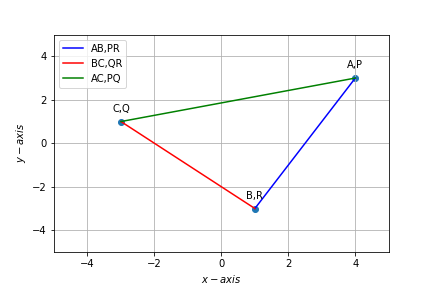
\includegraphics[scale=0.7]{triangle.png}
\end{figure}
\end{enumerate}
\end{document}
